\documentclass{article}

\usepackage{amsmath,amssymb}
\usepackage{xcolor}
\usepackage{tikz}
\usetikzlibrary{arrows.meta,decorations.markings}

\pagestyle{empty}

\begin{document}
	
	\begin{center}
		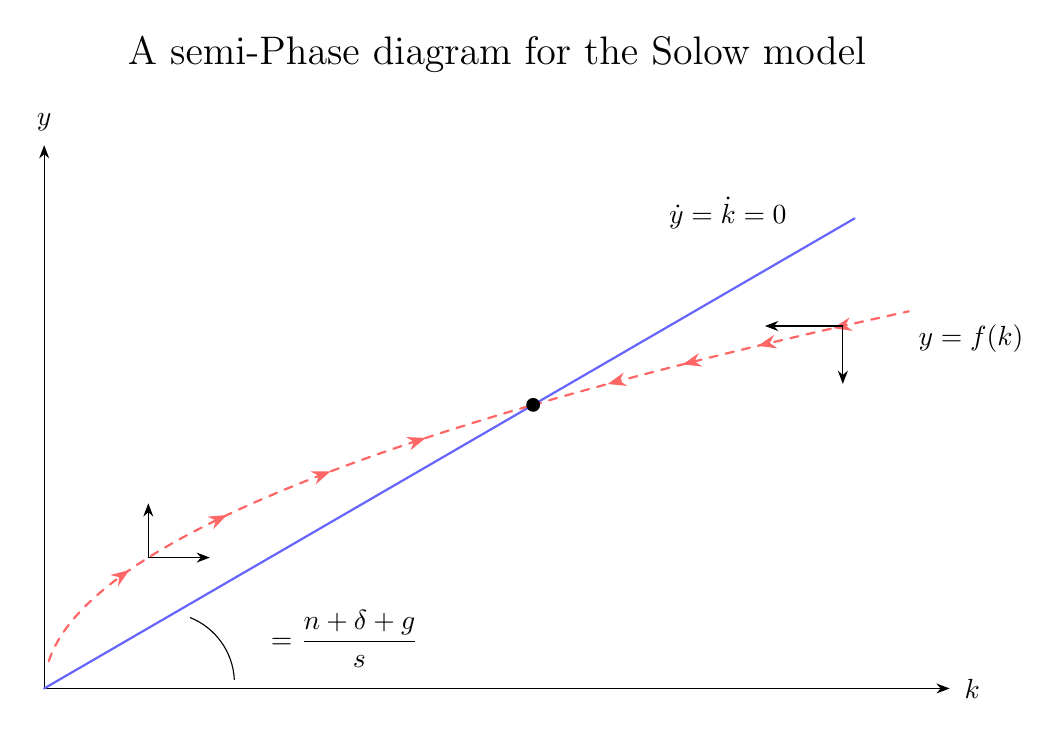
\begin{tikzpicture}[
			x=1.15cm,
			y=1.15cm,
			>=Stealth,
			line cap=round,
			line join=round,
			flowright/.style={
				postaction={decorate},
				decoration={
					markings,
					mark=at position 0.22 with {\arrow{Stealth}},
					mark=at position 0.42 with {\arrow{Stealth}},
					mark=at position 0.62 with {\arrow{Stealth}},
					mark=at position 0.80 with {\arrow{Stealth}}
				}
			},
			flowleft/.style={
				postaction={decorate},
				decoration={
					markings,
					mark=at position 0.20 with {\arrowreversed{Stealth}},
					mark=at position 0.40 with {\arrowreversed{Stealth}},
					mark=at position 0.60 with {\arrowreversed{Stealth}},
					mark=at position 0.80 with {\arrowreversed{Stealth}}
				}
			}
			]
			
			% 기본 수치
			\pgfmathsetmacro{\slopecoef}{0.58}
			\pgfmathsetmacro{\xstarval}{5.40}
			\pgfmathsetmacro{\ystarval}{\slopecoef*\xstarval}
			\pgfmathsetmacro{\rootcoef}{\slopecoef*sqrt(\xstarval)}
			
			\pgfmathsetmacro{\xleftcorner}{1.15}
			\pgfmathsetmacro{\yleftcorner}{\rootcoef*sqrt(\xleftcorner)}
			
			\pgfmathsetmacro{\xrightcorner}{8.82}
			\pgfmathsetmacro{\yrightcorner}{\rootcoef*sqrt(\xrightcorner)}
			
			% 축
			\draw[->] (0,0) -- (10,0);
			\draw[->] (0,0) -- (0,6);
			
			\node at (10.25,0) {$k$};
			\node at (0,6.25) {$y$};
			
			% 파란색 직선
			\draw[thick,blue!60] (0,0) -- (8.95,{8.95*\slopecoef});
			\node at (7.55,5.25) {$\dot y=\dot k=0$};
			
			% 빨간색 생산함수
			\draw[thick,dashed,red!60,flowright,domain=0.05:\xstarval,samples=160]
			plot (\x,{\rootcoef*sqrt(\x)});
			
			\draw[thick,dashed,red!60,flowleft,domain=\xstarval:9.55,samples=160]
			plot (\x,{\rootcoef*sqrt(\x)});
			
			\node[right] at (9.55,{ \rootcoef*sqrt(9.55)-0.3 }) {$y=f(k)$};
			
			% 교점
			\fill (\xstarval,\ystarval) circle (2.5pt);
			
			% ㄴ자 표시
			\draw[->] (\xleftcorner,\yleftcorner) -- (\xleftcorner,\yleftcorner+0.60);
			\draw[->] (\xleftcorner,\yleftcorner) -- (\xleftcorner+0.68,\yleftcorner);
			
			% ㄱ자 표시
			\draw (\xrightcorner,\yrightcorner) -- (\xrightcorner,\yrightcorner-0.55);
			\draw (\xrightcorner,\yrightcorner) -- (\xrightcorner-0.48,\yrightcorner);
			
			\draw[->] (\xrightcorner,\yrightcorner-0.22) -- (\xrightcorner,\yrightcorner-0.64);
			\draw[->] (\xrightcorner-0.22,\yrightcorner) -- (\xrightcorner-0.86,\yrightcorner);
			
			% 각도 표시
			\draw (2.10,0.10) arc[start angle=3,end angle=68,radius=0.78];
			\node at (3.32,0.55) {$=\dfrac{n+\delta+g}{s}$};
			
			% 제목
			\node at (5.0,7) {\Large A semi-Phase diagram for the Solow model};
			
		\end{tikzpicture}
	\end{center}
	
\end{document}